\chapter{Walkthrough}\label{ch:walkthrough}
\begin{figure}[ht!]
    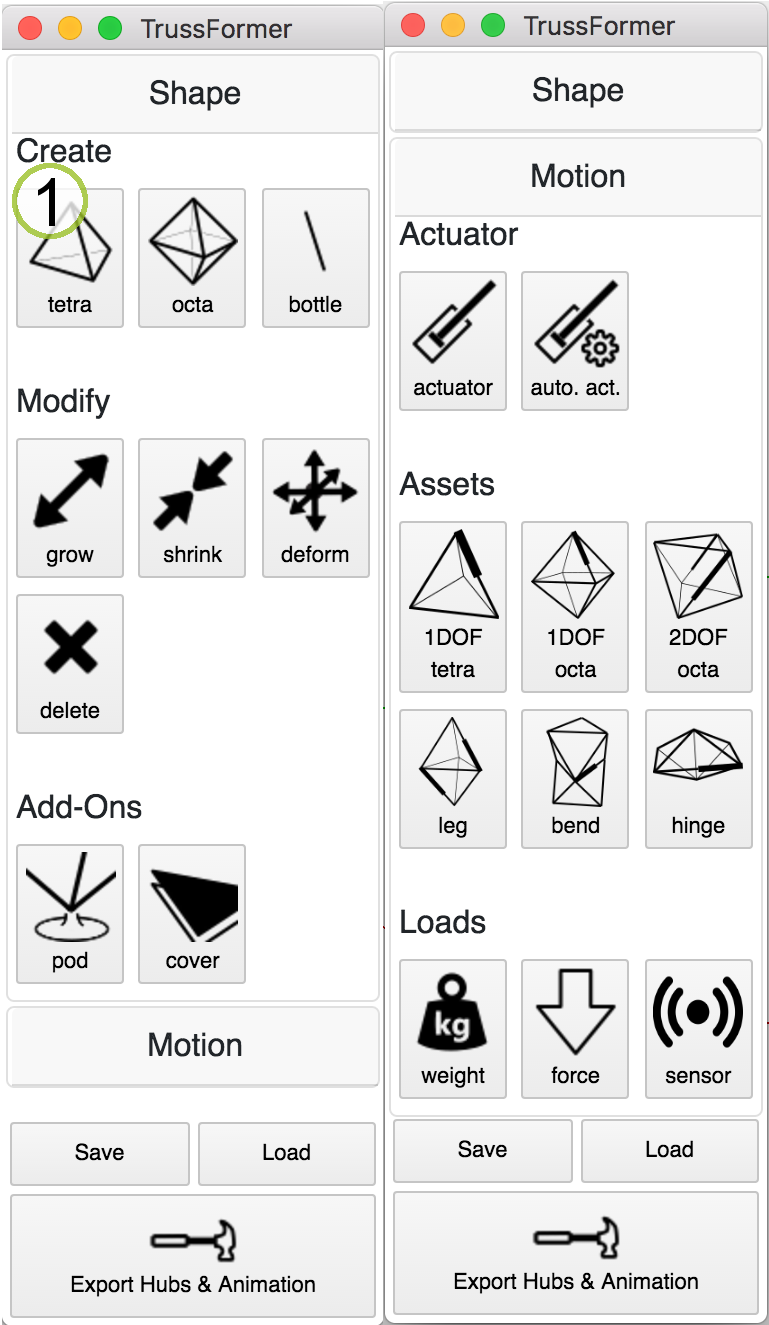
\includegraphics[width=.7\textwidth]{Walkthrough/UI.png}
    \centering
    \caption{TrussFormer's toolbar}
    \label{fig:toolbar}
\end{figure}
This chapter will present the functionalities of the system by showing the process of creating the T-Rex shown in Figure \ref{fig:examples} (c). This will include all steps from creating the static structure, over introducing animation, up to fabricating the final object.

\section{Designing Static Structures}
As shown in Figure \ref{fig:modelling_t-rex}, the T-Rex model was first created as a stable static structure. With the help of TrussFormer, the user can make sure that the object to be created is structurally sound before adding motion. The provided tools can create sturdy primitives that are attached to each other, deform the structure, and check forces acting on each part of the object.

\subsection{Primitives}
Users can use predefined and structurally stable primitives to create their objects. Our system provides tools for creating octahedra and tetrahedra (Figure \ref{fig:toolbar} (1)). These truss primitives consist entirely of triangular faces, which is an essential property for stable objects and widely used in heavy industry and architecture, e.g. for cranes or bridges.

\subsection{How they are used}
The primitives can be attached to existing triangle faces, as seen in Figure \ref{fig:modelling_t-rex} or placed on the ground. If necessary, our system can also create single links between two nodes using the bottle link tool (2).\\
The form of the structure can be tweaked as desired by using the grow and shrink tool (3). These tools elongate or shorten edges, deforming the structure in such a way that the truss structure stays intact. As our PET bottle system only allows three different sizes of edges (two big bottles, one big and one small bottle, two short bottles), we elongate the connecting parts on the nodes. The grow and shrink tools will change the length of the \textit{elongation} as long as a different bottle configuration is possible. So, if the users wants to shorten a certain edge a lot, the shrink tool will determine, that it should become a short-short bottle link and adapt the elongations accordingly. The deform tool (4) does a similar job, but rather than working on edges, this tool can move nodes.\\
For settling the object on the ground or placing a cover on a triangle face, TrussFormer also provides a pod tool (5). Pods provide a flat surface on nodes that stands proud of the curved bottle bodies, making it easier to have a firm and level stand. Nodes that have a pod will not be changed by the modifying tools.

\begin{figure}[ht!]
    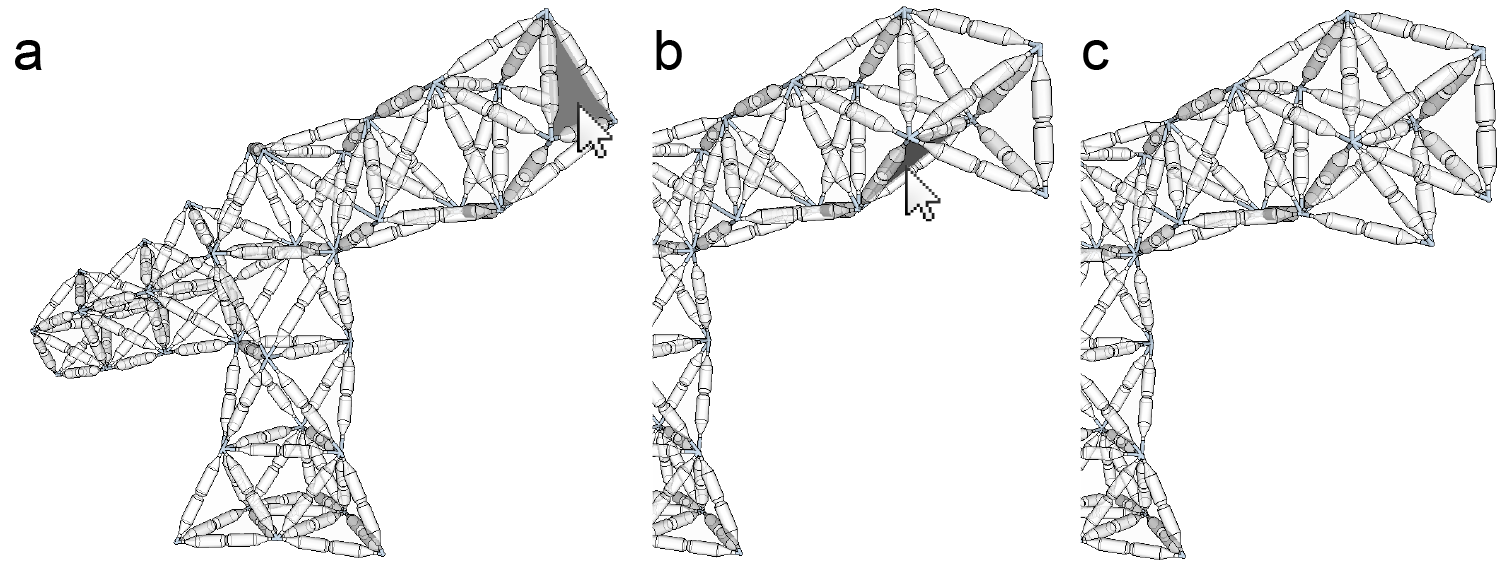
\includegraphics[width=\textwidth]{Walkthrough/modeling_dino_(trussfab)-01.png}
    \centering
    \caption{Modeling the static shape of the T-Rex. Here, the user creates the jaws of the T-Rex by attaching tetrahedron primitives through the steps (a, b, c).}
    \label{fig:modelling_t-rex}
\end{figure}

\subsection{Check static forces}
Using the animation pane, the user can determine static forces acting on the structure. TrussFormer provides tools for adding weight to the structure. In the case of our T-Rex, users might want to add decoration with a weight of 5 kg to its head. They select the \textit{Add Weight Tool} (6) and click a node. After that, they use the \textit{Play button} (Figure \ref{fig:animation} (12)) in the animation window. Our built-in simulation will visualize occurring forces and check if the structure is capable of withstanding the additional weight.

\section{Adding Movement to the Structures}
Movement is added to the structure by placing special physics edges. These edges act like linear actuators - struts that can extend and retract in a straight line. There are multiple methods for placing these actuators, ranging from a fully-automated way to manual placement.

\subsection{Automatic Actuator Placement}
The automated way works by demonstrating a desired movement. The user selects the \textit{Demonstrate Movement Tool} (6), clicks a node that should experience a certain movement and drags a line to the desired end position, as seen in Figure \ref{fig:demonstrate_movement}. TrussFormer will then search for an actuator that brings the node closest to the desired position and turns the resulting edge into an actuator. The tool runs through all edges of the structure, replacing one after another with an actuator and simulates the resulting movement in the background. The actuator that solves the problem the best will be placed.
\begin{figure}[ht!]
    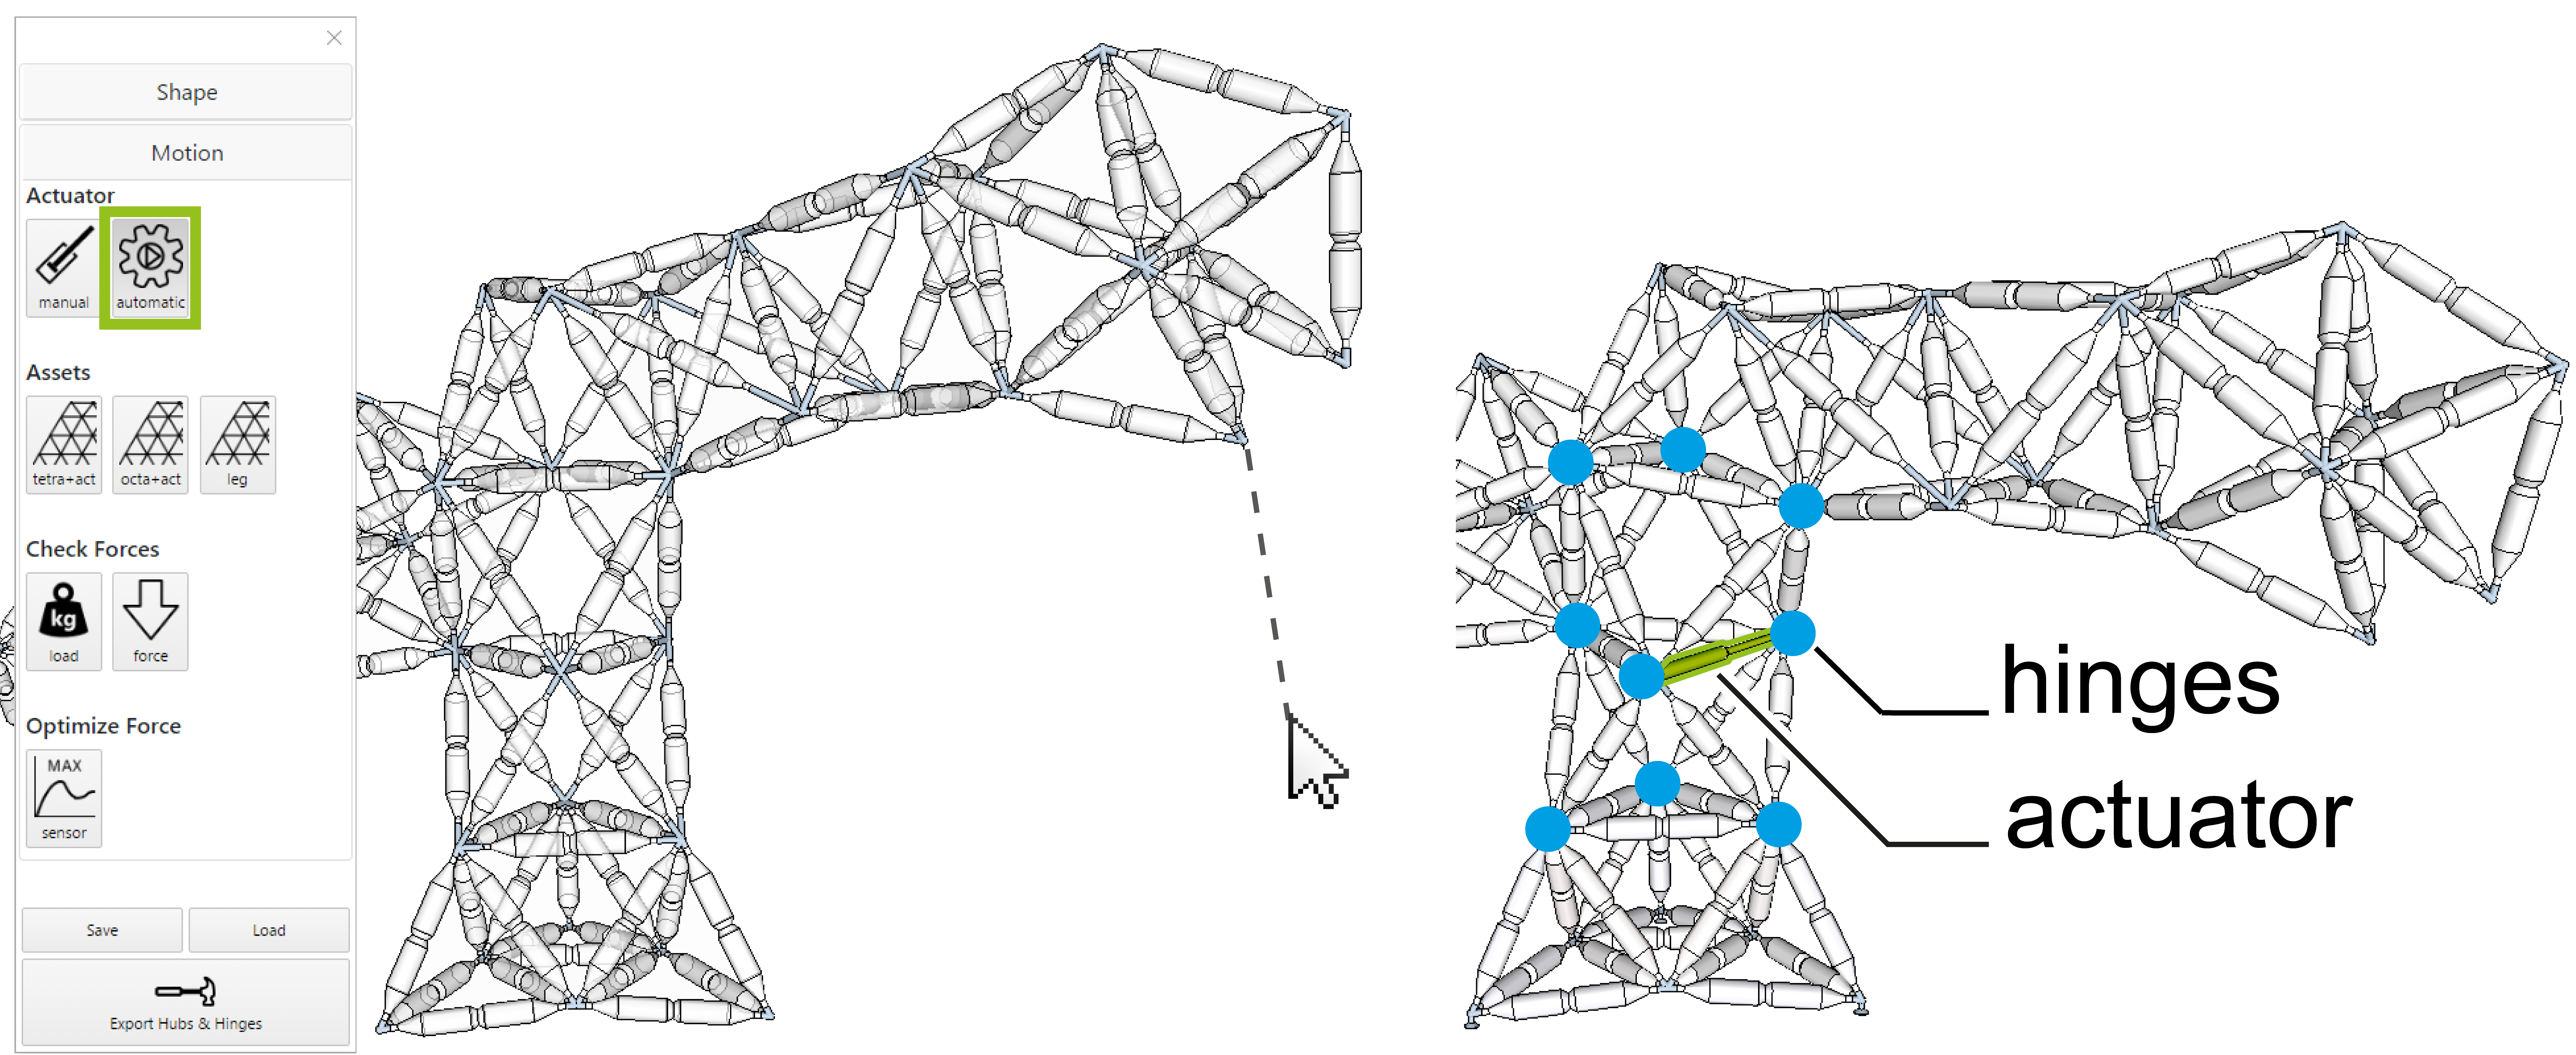
\includegraphics[width=\textwidth]{Walkthrough/demonstrate_movement_tool.png}
    \centering
    \caption{(a) The user selects the demonstrate movement tool and pulls the T-Rex head downwards. (b) TrussFormer responds by adding an actuator to the T-Rex body so that it is capable of performing this type of motion. At this point the system also places 9 hinging hubs to enable this motion (marked with blue dots).}
    \label{fig:demonstrate_movement}
\end{figure}

\subsection{Placing Primitives}
Another way to add movement is to use predefined dynamic assets. It can be difficult for a user to fully grasp how an actuator will move the whole object. We encapsulated often-used assets into tools (7). These assets connect to the rest of the structure through a dedicated triangle surface. Because the motion is localized in this asset, the result in the bigger structure is easier understandable. A selection of assets is shown in Figure \ref{fig:dynamic_assets}\\
Instead of using the demonstrate movement tool to create the nodding motion of the T-Rex, a ``bending'' double-octahedron, as seen in Figure \ref{fig:dynamic_assets} (f) could have been used in the vertical body part.
\begin{figure}[ht!]
    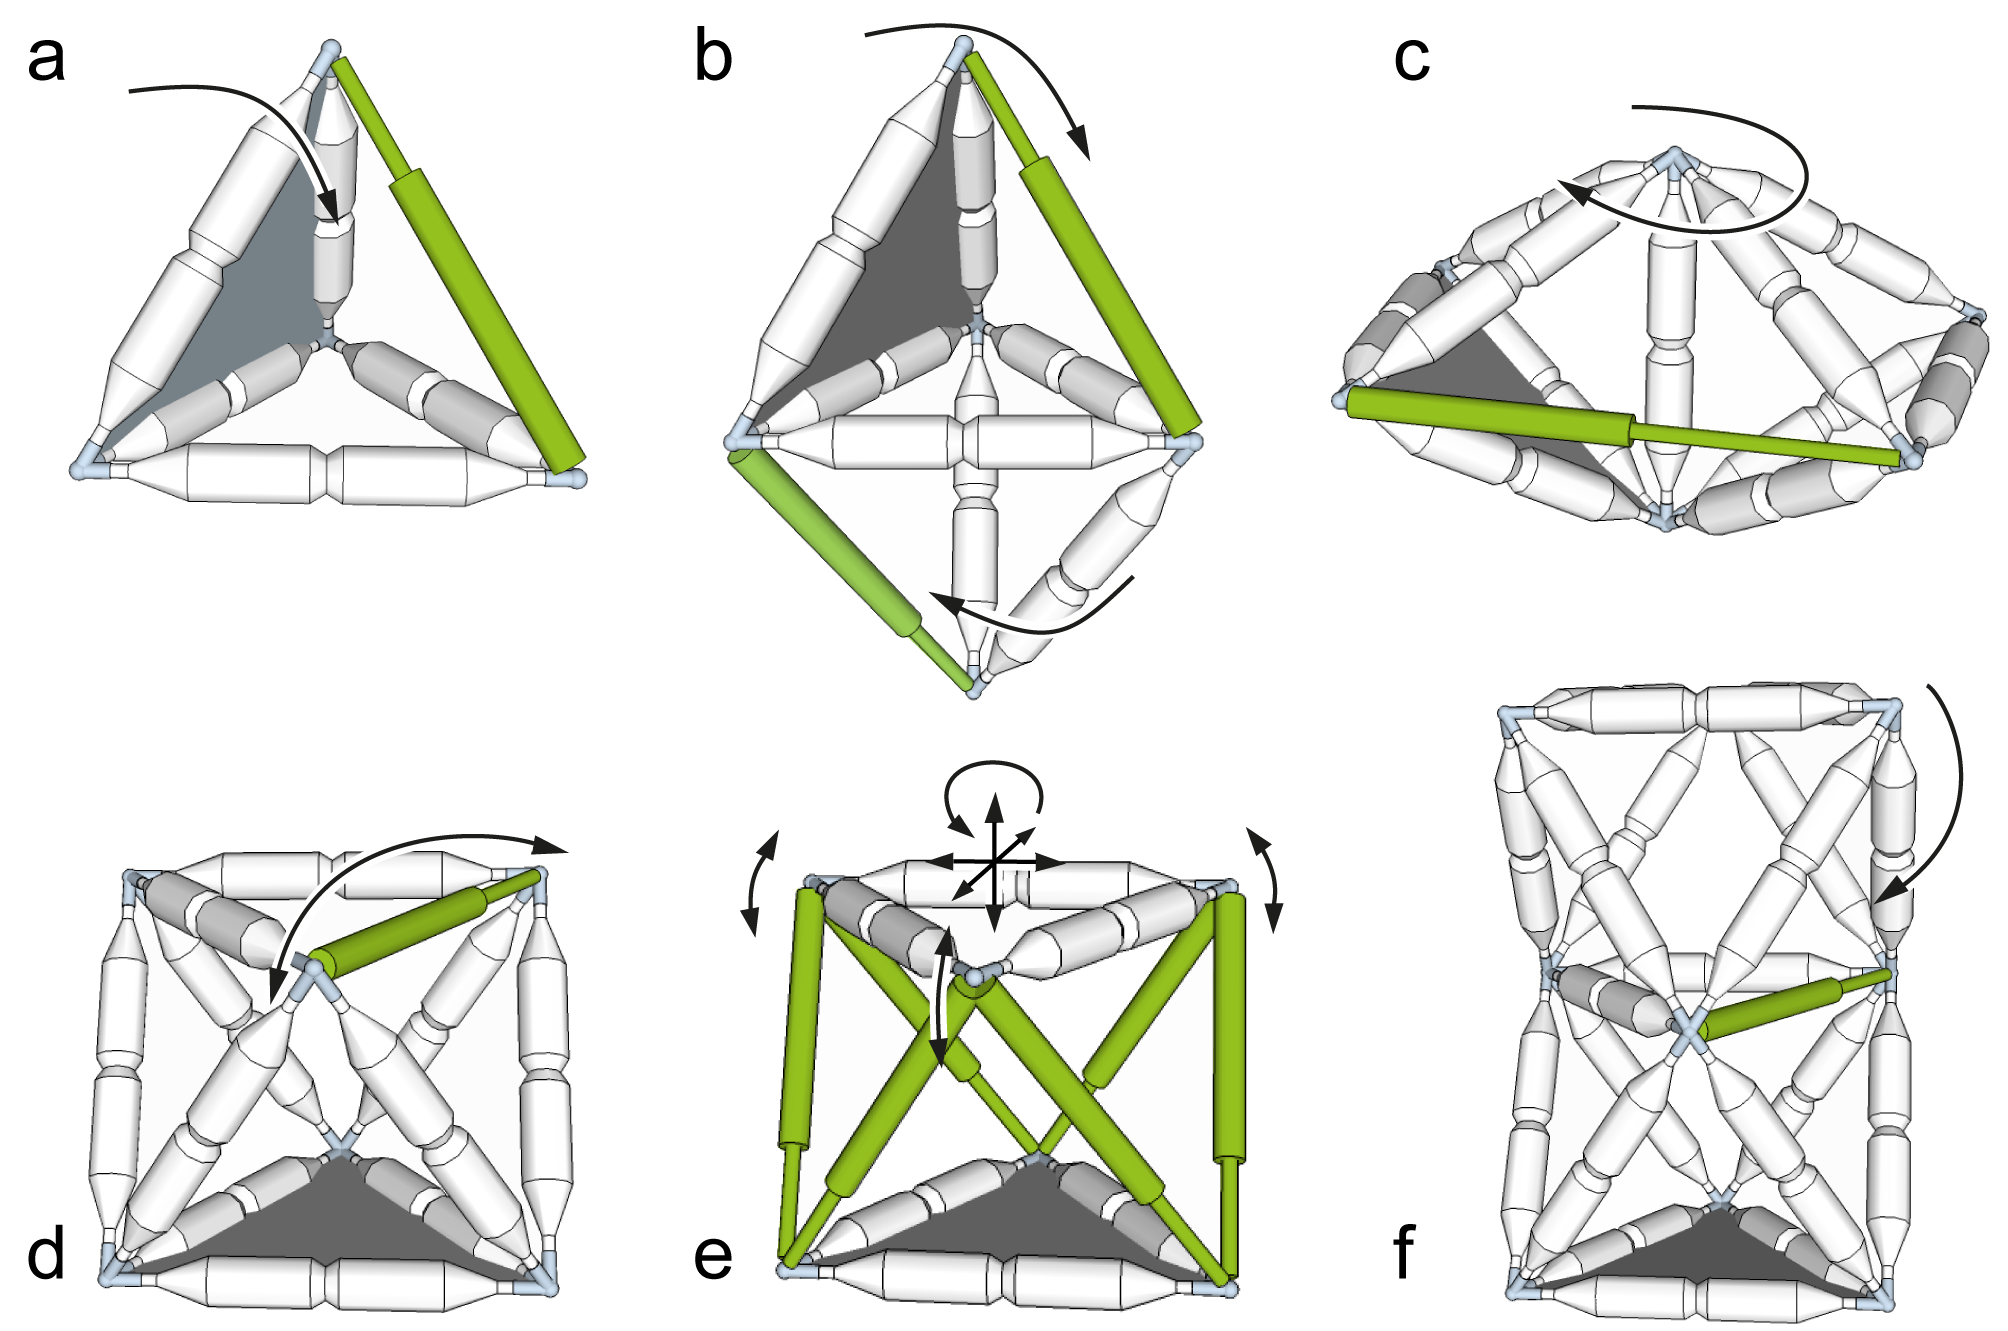
\includegraphics[width=\textwidth]{Walkthrough/assets_white-01.png}
    \centering
    \caption{A selection of assets: (a) tetrahedron with 1DoF, (b) “robotic leg” asset, (c) hinging tetrahedron, (d) octahedron with 1DoF, (e) Stewart platform (6DoF), and (f) double-octahedron performing “bending” motion.}
    \label{fig:dynamic_assets}
\end{figure}

\subsection{Manual Actuator Placement}
The manual actuator placement requires the most knowledge about the resulting motion. It is, however, the most flexible way to create movement. The user can choose the \textit{actuator tool} (8) to turn any edge into or connect two nodes with an actuator. This can be done by clicking on the desired edge or selecting two nodes to be connected. Transforming an existing edge is usually the desired use case, as the introduction of more edges (by connecting two previously unconnected nodes) tends to make the truss more stable and can prevent motion altogether. Turning an edge into an actuator essentially removes this edge and adds a degree of freedom.
\begin{figure}[ht!]
    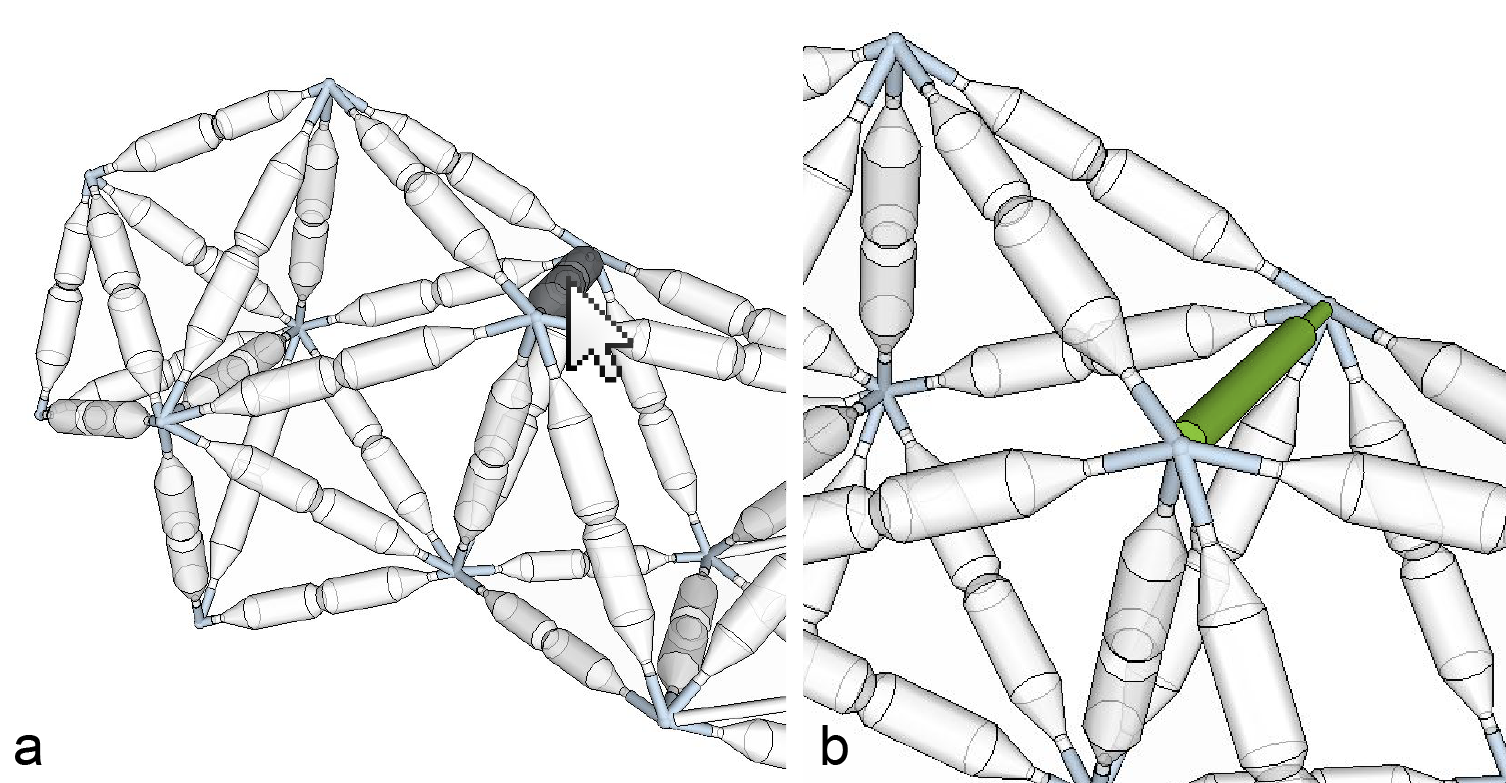
\includegraphics[width=\textwidth]{Walkthrough/manual_actuator_placement.png}
    \centering
    \caption{The turn edge to actuator tool allows users to turn any edge into an actuator. Here the user replaces one edge in the T-Rex’s head to make its jaws move.}
    \label{fig:manual_actuator}
\end{figure}

\subsection{Stability Check}
During the placement of actuators, TrussFormer verifies that the mechanism is structurally sound. The system finds the safe range of actuation in the background, i.e. how far an actuator can extend without damaging the structure, by simulating the occurring forces in a range of positions. Damage can occur if the structure falls over, hits the ground with too much speed or if too much force is exerted on a structural element, such as an edge, as illustrated in Figure \ref{fig:check_poses}. To do this, TrussFormer iteratively extends each actuator and observes the forces. If the force exceeds a preset limit, the last safe actuation range is stored in the actuator. The user will then not be able to over-actuate this actuator.\\
To completely prevent breaking, this process would have to be done for each combination of actuators. As this does not scale well with an increasing number of actuators in the system, we perform this step for each actuator individually. An additional security check is done while the user tries out the motion manually, as explained in the next section.
\begin{figure}[ht!]
    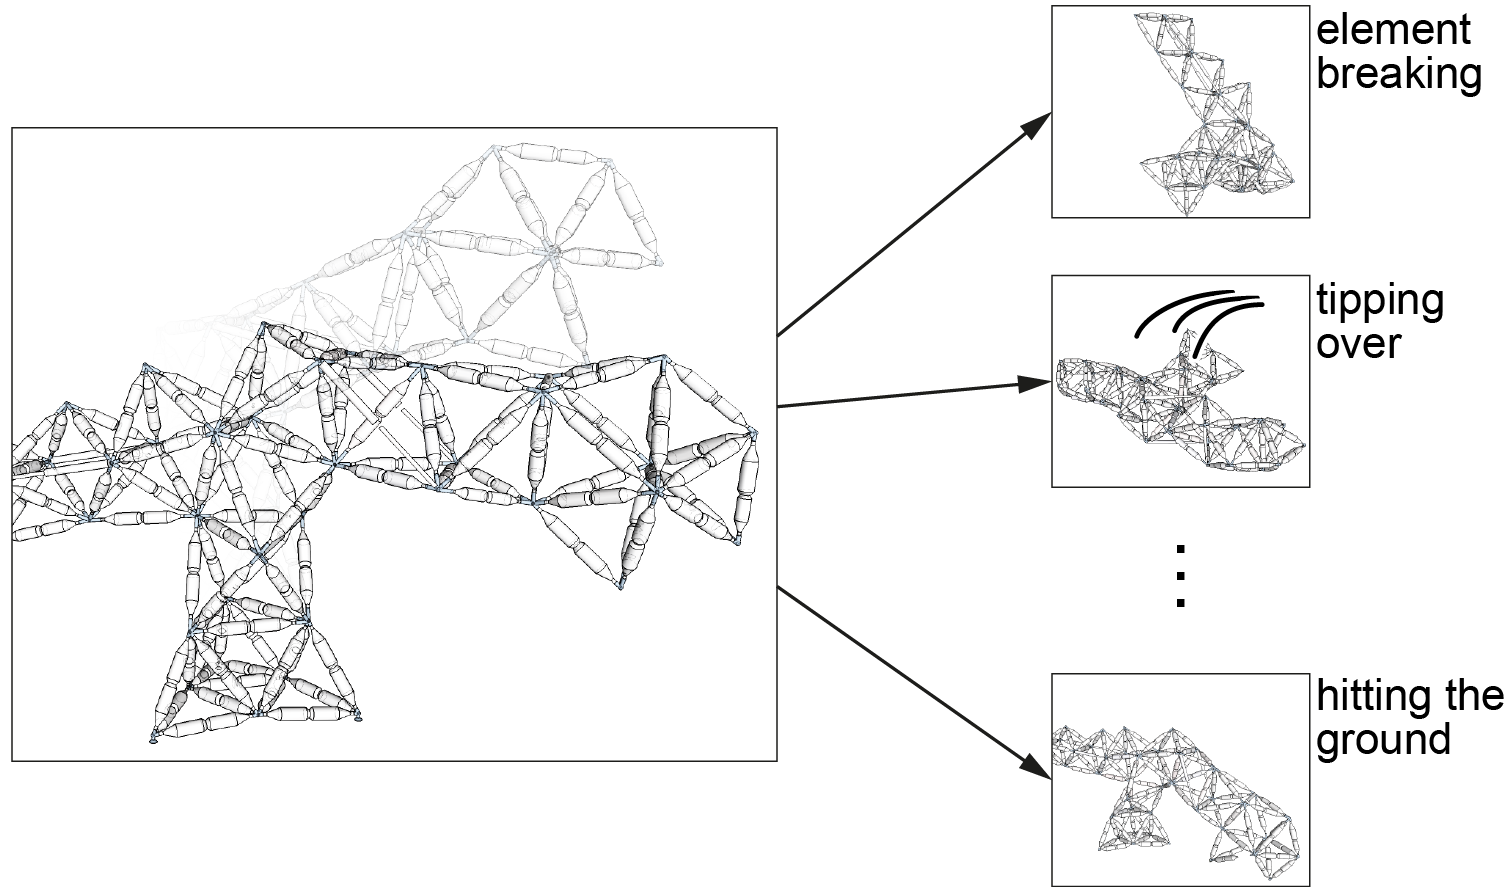
\includegraphics[width=\textwidth]{Walkthrough/check_poses.png}
    \centering
    \caption{In the background, TrussFormer tests each actuator to see if its extension leads to invalid configurations, such as the structure falling over, hitting the ground, or encountering broken structural elements.}
    \label{fig:check_poses}
\end{figure}

\section{Animation}\label{sec:animation}
The user can actuate the physics links in two different ways. The \textit{animation window} provides a slider for manual movement (Figure \ref{fig:animation} (9)), as well as an animation pane which allows placing keyframes (10) and provides two playback modes (11). All actuators have an actuator group assigned to them. Per default, an actuator is placed in its own, empty group. Using the actuator tool (Figure \ref{fig:toolbar} (8)), already used for placing actuators, this group can be changed. This is indicated by the actuator changing its color.\\
The control elements of the animation window always work on the whole group. The color of the animation line indicates which group will be actuated by either the slider or the keyframes.
\begin{figure}[ht!]
    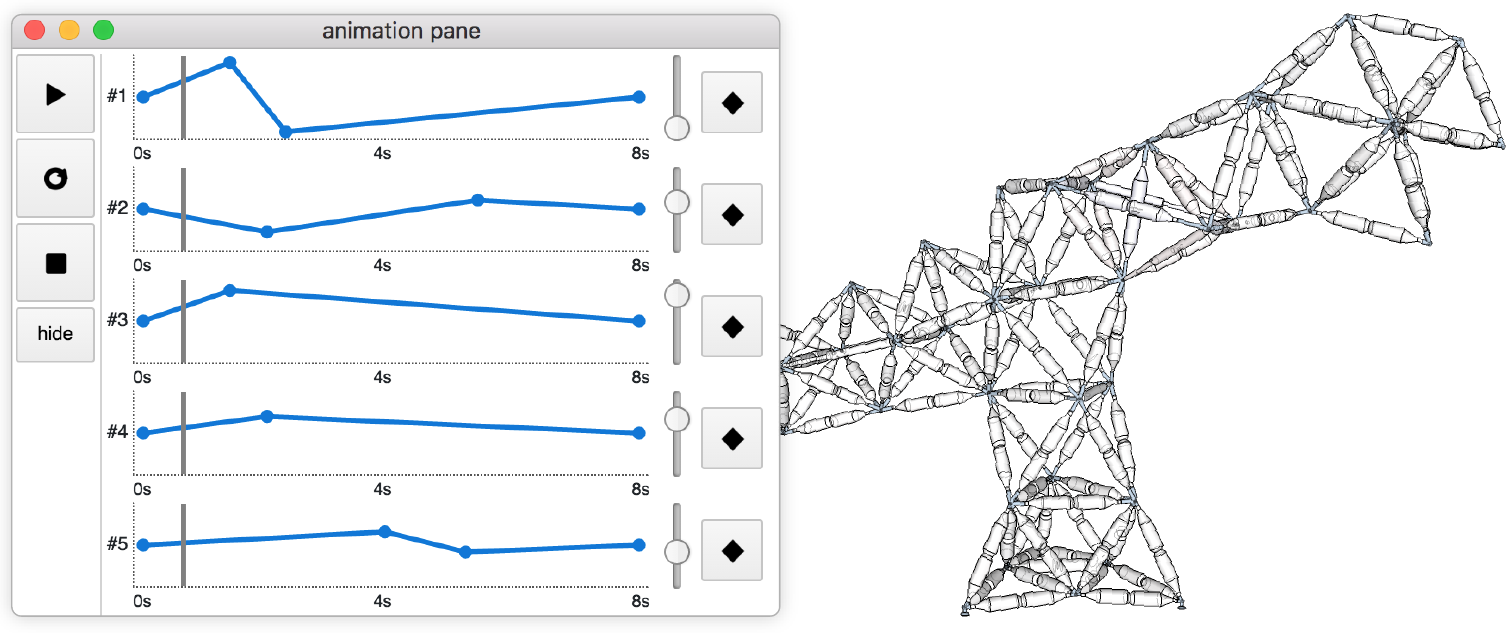
\includegraphics[width=\textwidth]{Walkthrough/animating_the_structure.png}
    \centering
    \caption{Animating the structure. Users sets the desired pose using the sliders in the animation pane and orchestrate the movement by placing key-frames on the timeline. Each timeline controls actuators with the same color.}
    \label{fig:animation}
\end{figure}
To add a key\-frame to the animation pane, first the slider has to be moved to the desired position. The object will start to move according to the sliders position - if the slider is at the top, the actuator will be fully extended and vice versa. That way, the user can visualize the extent of the movement. If the user is satisfied, the indicator line can be moved to the desired position in the timeline and the diamond button is pressed to add this keyframe to the animation.

\subsection{Checking Dynamic Forces}
If the structure fulfills the desired motion, the user will want to check if the forces created during executing it will not exceed the breaking force of the object. A lot of factors play a role in the formation of forces. These range from weight forces over lever forces to inertial forces. TrussFormer aids the user in detecting weak points and force peaks during a motion in different ways.\\
TrussFormer's tools provide the possibility to constantly monitor the forces that occur during interactive movement of the structure. In simulation mode, all edges will be colored red or blue in increasing intensity the higher the force on them is. Red indicates compression force, while blue means tension force. A completely white color indicates a force of $0 N$. These tension forces are automatically calculated by the built-in physics engine.\\
As shown in Figure \ref{fig:fix_breaking} (a) the user creates an animation that moves the T-Rex body down and up again. (b) While TrussFormer plays the animation, it calculates the forces. The change from the downwards motion to going up again causes a lot of contraction force on the edges on the front body side. The neck of the T-Rex acts as a lever, which leads to very high inertial forces. This motion eventually exceeds the breaking limit of the structure, (c) causing the construction to fail. The time of breaking is indicated in the animation pane by a red vertical line. This failure is hard to predict by the user, because inertial forces can be multiple times higher than the static forces, checked during the creation of the T-Rex. (d) TrussFormer helps the user to fix the motion. A popup is opened providing two possibilities (Figure \ref{fig:correcting_animation}): fixing the animation by reducing the speed or reducing the motion. If the first option is chosen, TrussFormer will elongate the animation sequence for all piston groups. This results in a slower movement and less force on the structure. The second option will keep the length of the animation, but move the keyframes closer to the center line. The amplitude of the motion will be decreased.\\
Both versions will reduce the acceleration of the structure. The force formula $F = m * a$ shows, that the force increases proportionally with the acceleration, as the mass is constant in the structure. Reducing acceleration also reduces the force.
\begin{figure}[ht!]
    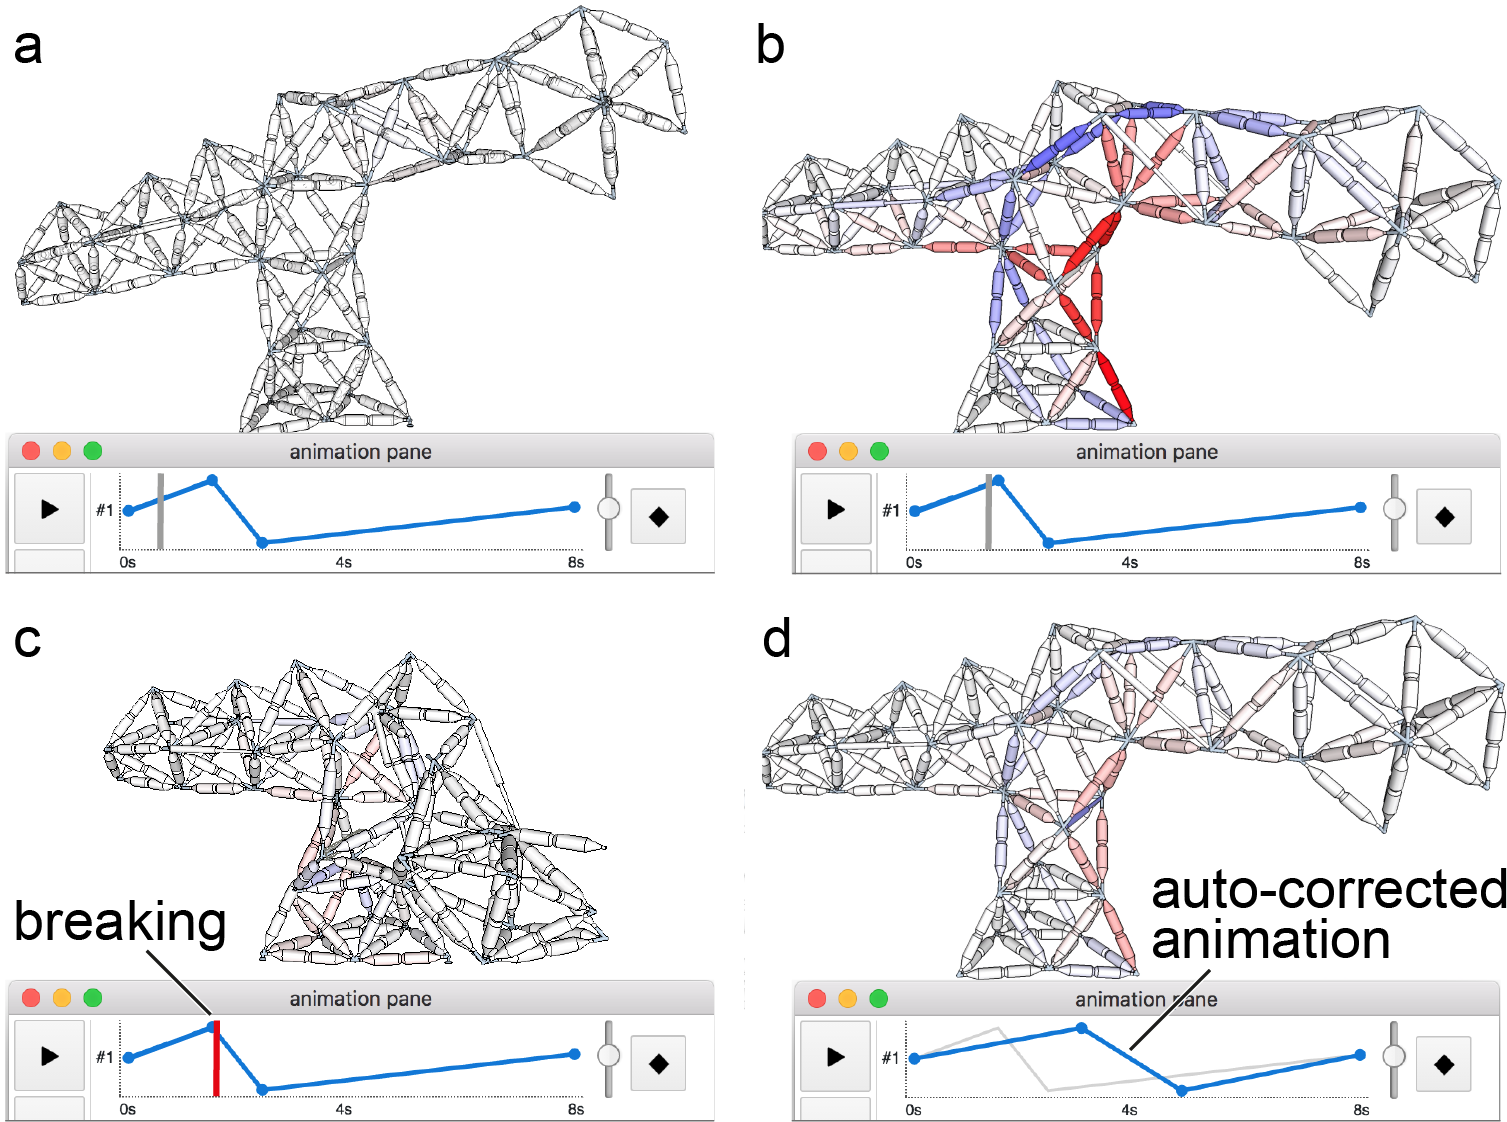
\includegraphics[width=\textwidth]{Walkthrough/forces-01.png}
    \centering
    \caption{TrussFormer verifies that the structure can withstand the inertial forces resulting from the programmed animation. (a-b) The forces in the T-Rex increase with the movement. (c) The structure breaks when the direction of the movement changes rapidly. (d) TrussFormer resolves this by making the movement slower.}
    \label{fig:fix_breaking}
\end{figure}
\begin{figure}[ht!]
    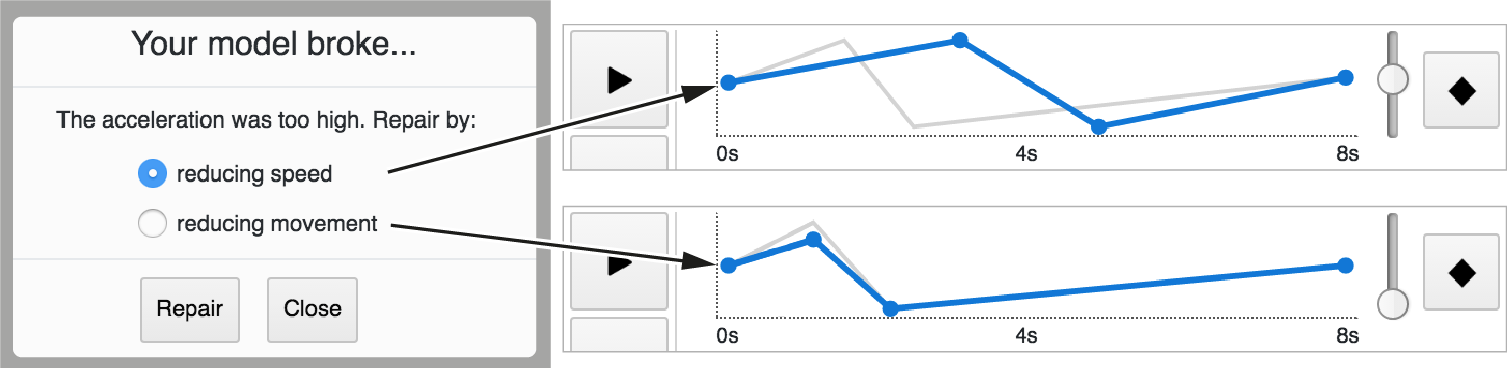
\includegraphics[width=\textwidth]{Walkthrough/auto_correcting_animations.png}
    \centering
    \caption{If the user-defined animation breaks the model, TrussFormer offers to automatically reduce the speed or the motion range.}
    \label{fig:correcting_animation}
\end{figure}

On top of the coloring of edges, the user can also use the \textit{sensor tool} (12). This tool can be used on a single edge to observe it more closely. The force data on an edge with a sensor will be recorded and visualized over time in a chart. The sensor tool also works on nodes, visualizing speed and acceleration data, instead of force. The result can be seen in figure \ref{fig:sensor}.\\
\begin{figure}[ht!]
    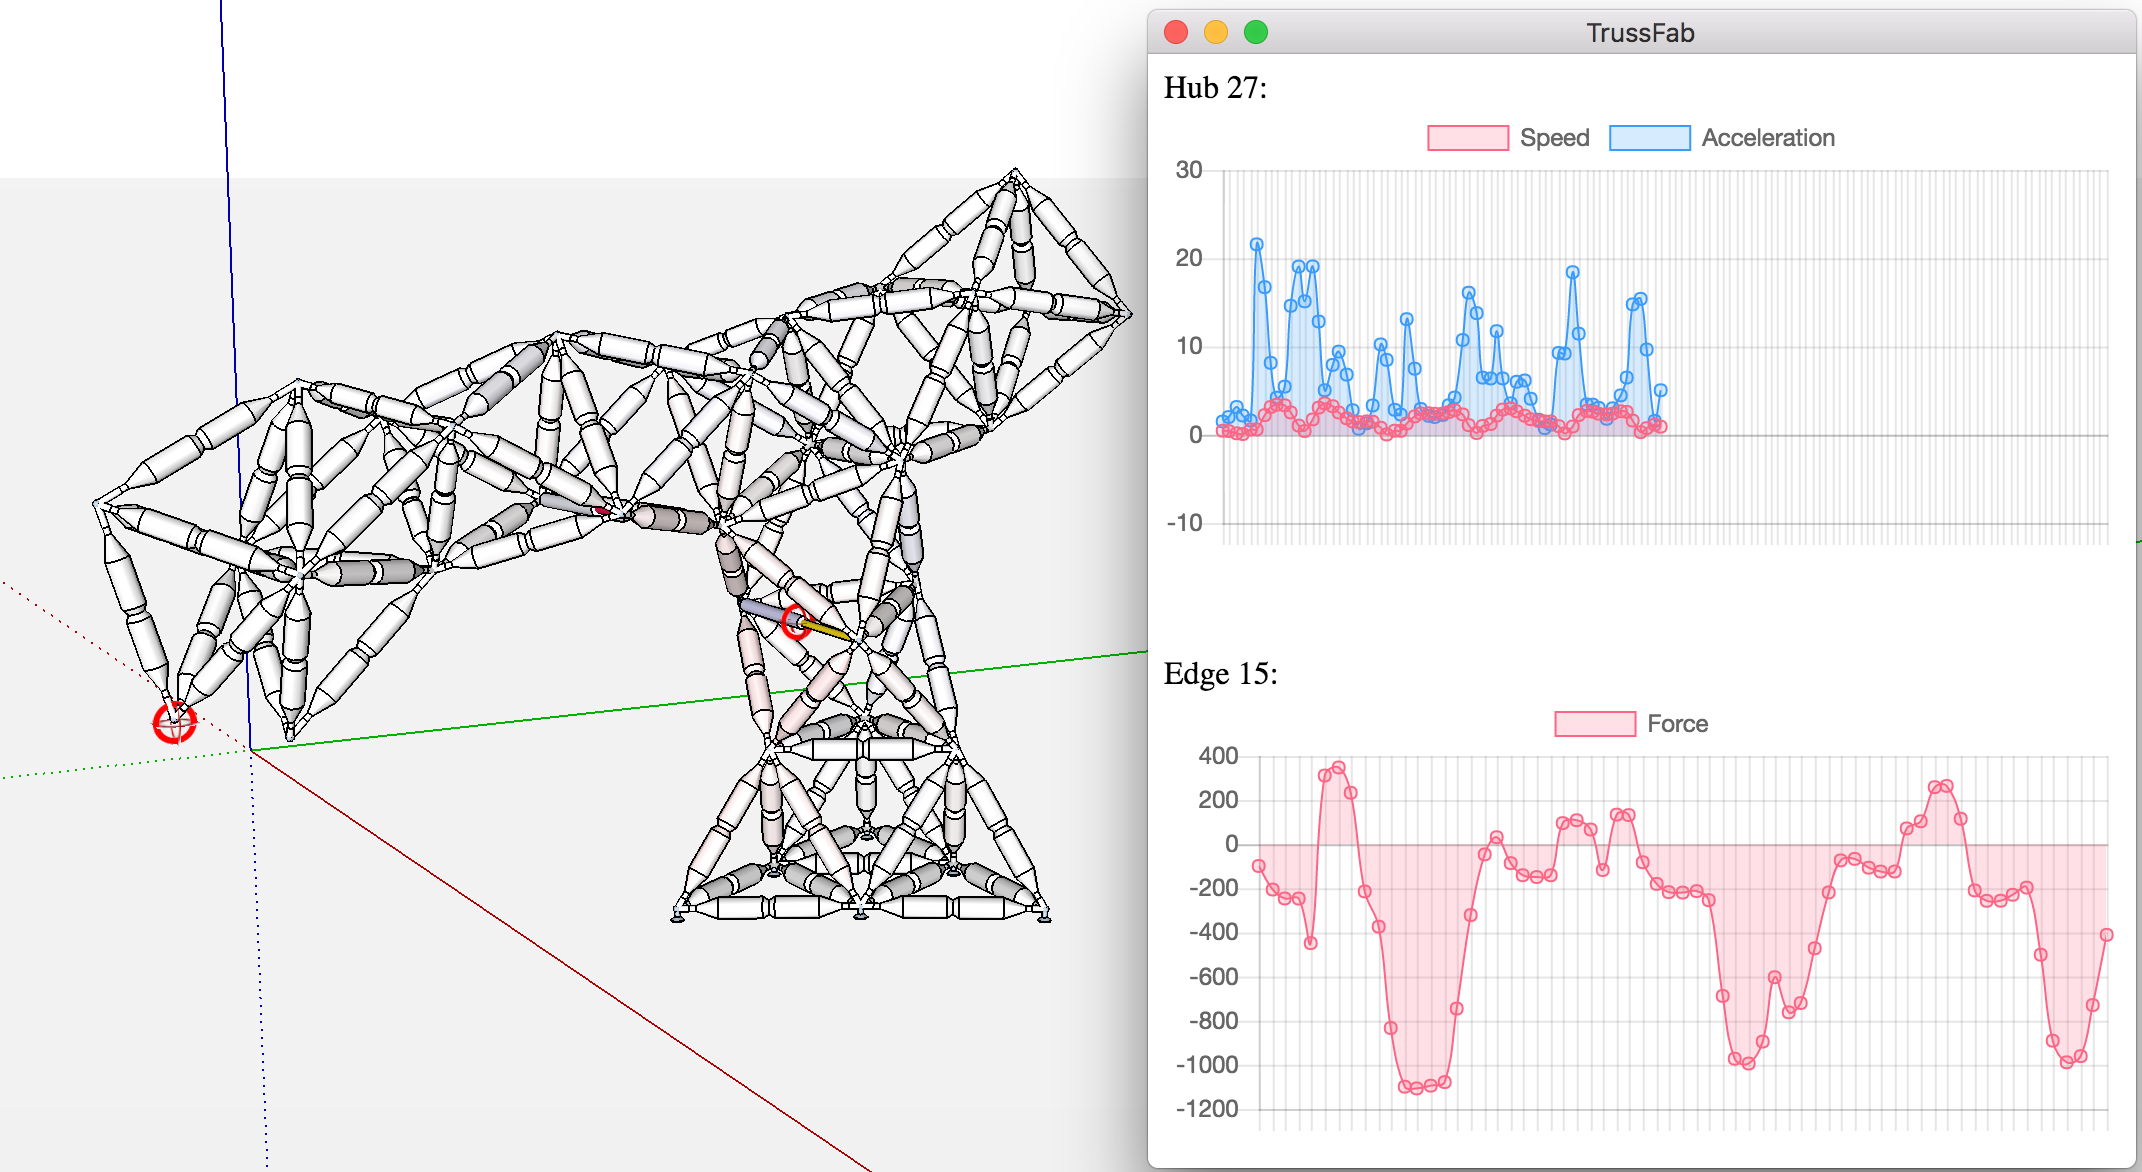
\includegraphics[width=\textwidth]{Walkthrough/sensor.png}
    \centering
    \caption{A sensor measures the force on the central actuator, and speed and acceleration on a node at the ``nose'' of the T-Rex}
    \label{fig:sensor}
\end{figure}

\section{Fabrication}
After the object was sufficiently tested in the editor, users want to print the connectors and assemble the final object. To do this, TrussFormer will calculate which connections need to move in the printed object and which can be static. It also takes into account constraints, such as the minimum distance from a bottle neck to the center of a hinge, which might otherwise restrict movement. This process will be explained in detail in Section \ref{sec:hinge_placement_impl}.

\subsection{Export}
When users are satisfied with their design (structure, movement, and animation), they click the \textit{fabricate} button (13). This will trigger TrussFormers' hinge generation procedure and create files which can be used for 3D printing. In order to control the structure the same way as in the animation pane, the animation will also be exported in an Arduino-readable format. Instructions for building will also be provided.
\begin{figure}[ht!]
    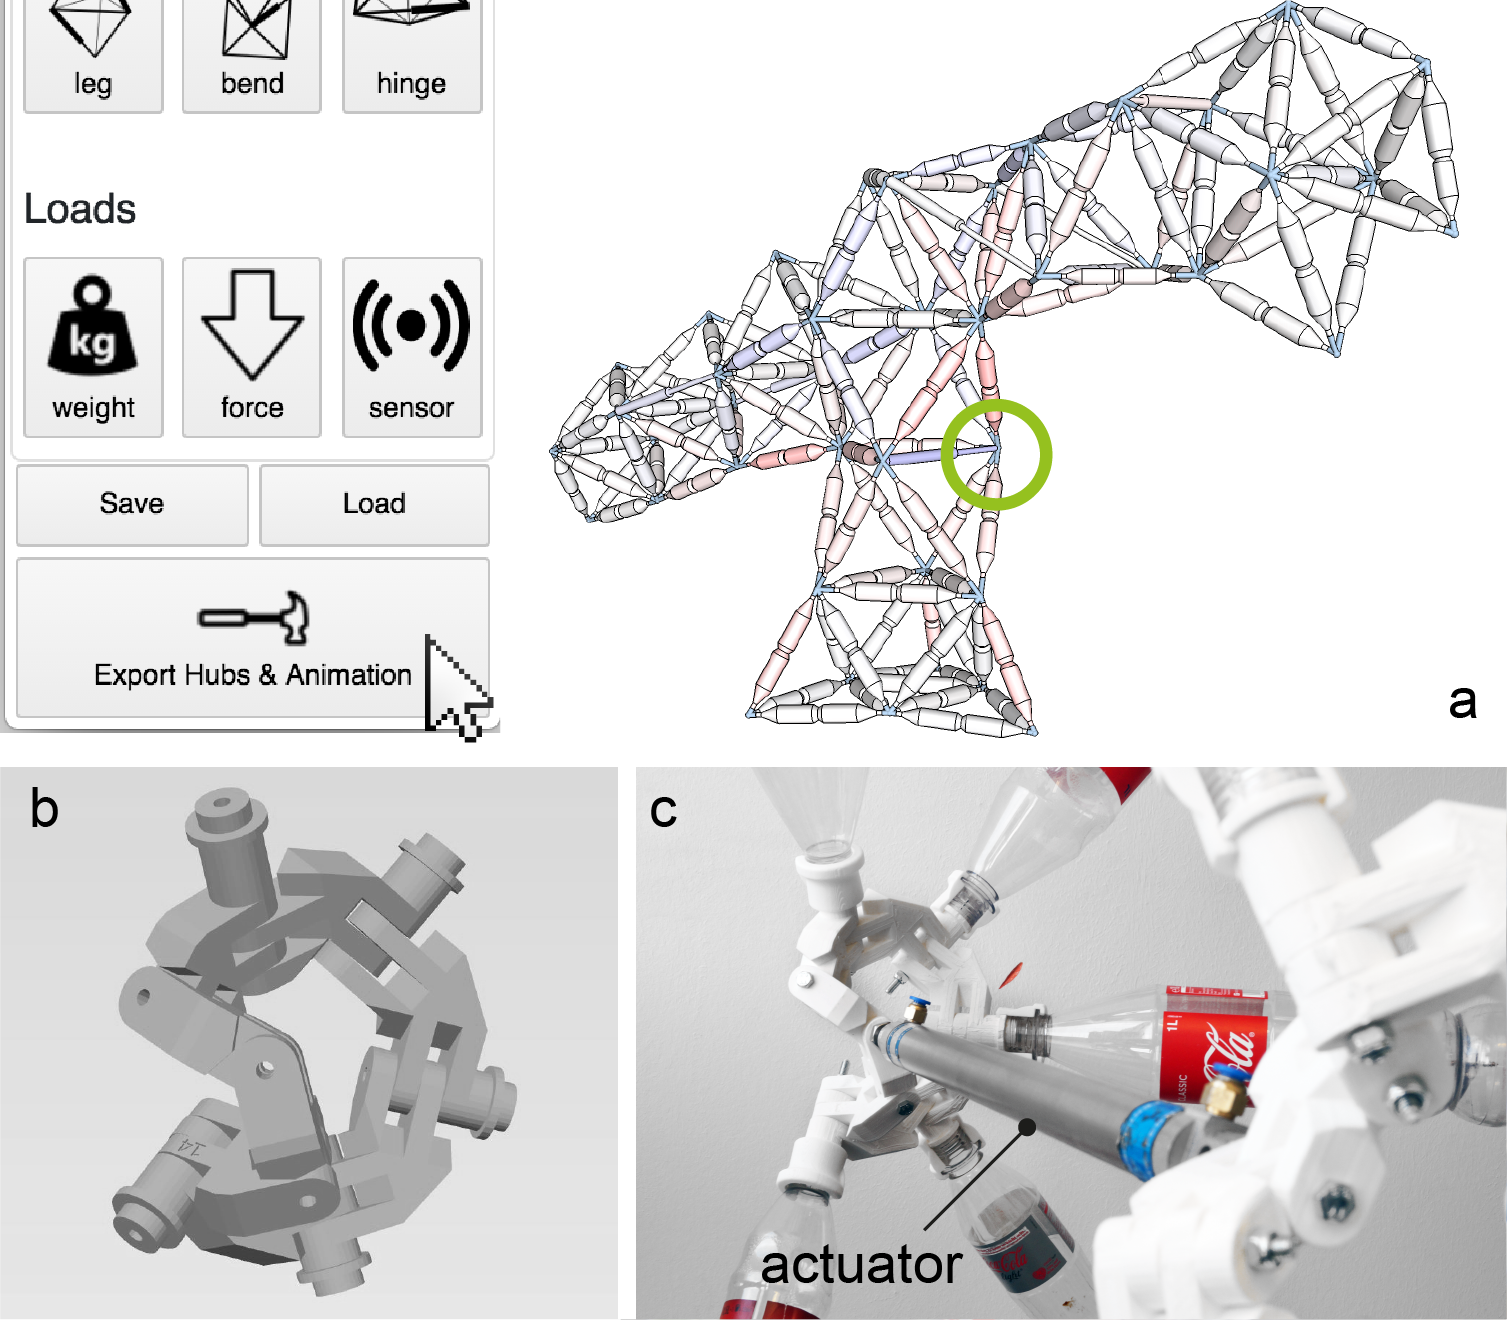
\includegraphics[width=\textwidth]{Walkthrough/export_and_hinges.png}
    \centering
    \caption{(a) To fabricate our T-Rex model, TrussFormer exports: (b) the appropriate 3D printable hinging-hubs for fabricating the structure, (c) and the actuator specifications that inform the users which one to buy. TrussFormer also exports the animation sequence for an Arduino.}
    \label{fig:export_and_hinges}
\end{figure}

TrussFormer's hinge generation procedure will analyze the structure, ensuring that the final object has the maximum possible movement and creates 3D printable hub geometries. The T-Rex consists of 42 3D printed hubs and 135 unique hinge pieces. An example can be seen in Figure \ref{fig:export_and_hinges}.\\
Next, the animation pattern is exported to Arduino code. The user can upload this code directly to their micro controller.\\
As a last step, specifications containing information about the force, speed and motion range of the actuators necessary for achieving the desired animation pattern, are created. Actuators that fulfill these requirements can be obtained as standardized components. The specifications also include information about the number and size of screws needed for assembly.

\subsection{Printing the Parts}
Each exported file represents a single part in the structure. These files can easily be converted to \textit{.stl} files, which are typically used for 3D printing. Using a 3D printing software, the 3D objects can be arranged and sent to a 3D printer. Printing of one hinge part using an UltiMaker 3 printer takes about 40 minutes.

\subsection{Assembling the Structure}
The resulting hubs and hinges contain an ID system for easy assembly. Each part of a node has the node ID printed on. That way it is easy to find out which hinge-parts belong together. Additionally, each edge elongation contains the id of the connected edge. Two hinge parts with the same node ID and edge ID will be connected, as can be seen in Figure \ref{fig:hinge}.\\
Two connectors with different node IDs but the same edge IDs will be connected by an edge.
\begin{figure}[ht!]
    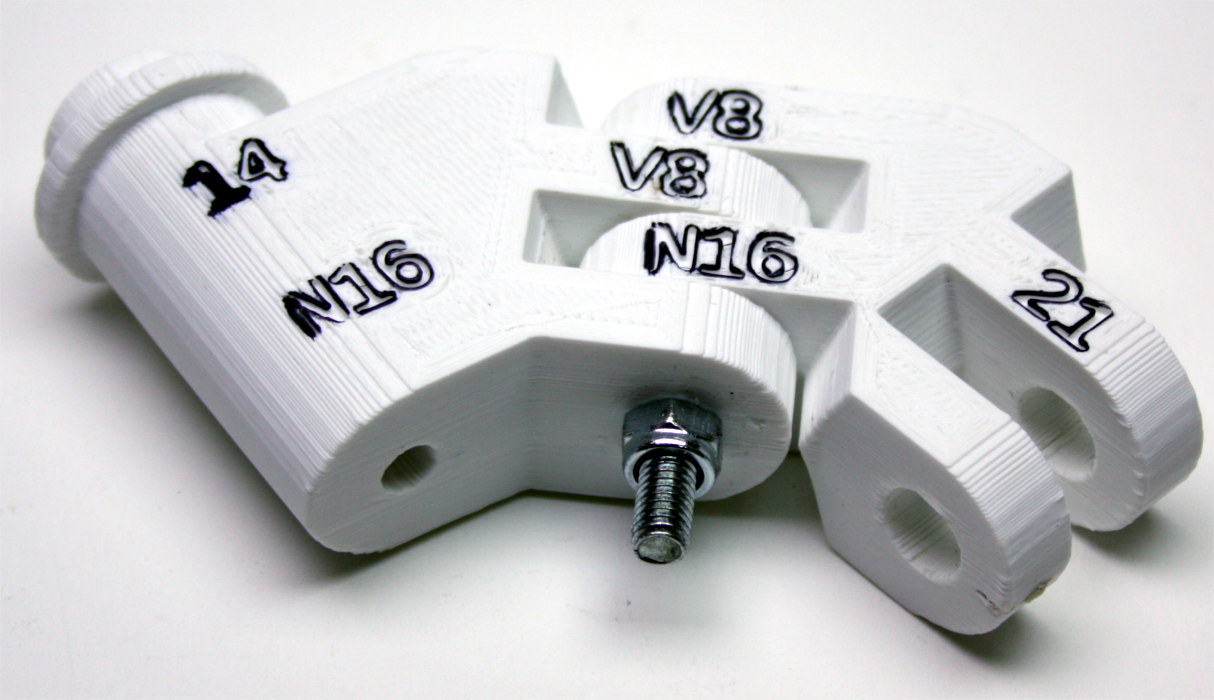
\includegraphics[width=\textwidth]{Walkthrough/hinge.png}
    \centering
    \caption{Two connected hinge parts. Both belong to hub 16 (\textit{N16}). Their connection has the ID \textit{V8}, indicating that this is an intermediate hinge connection (explained in Section \ref{sec:hinges}). The left connector will be linked with edge 14.}
    \label{fig:hinge}
\end{figure}
